% Gráfico: Taxa de Destruição - Nodes Left
\begin{figure}[htbp]
\centering
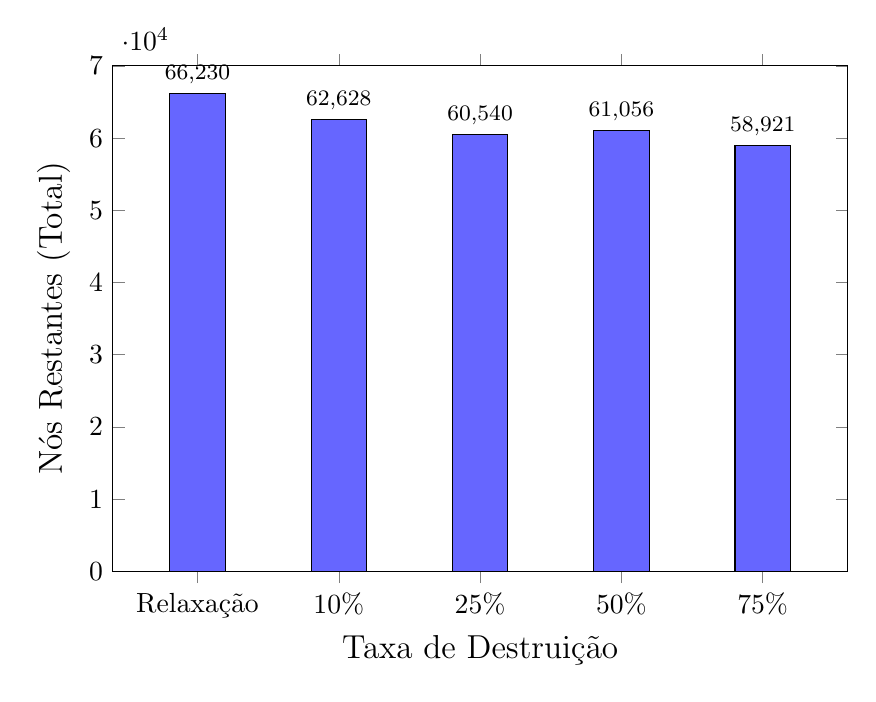
\begin{tikzpicture}
\begin{axis}[
    ybar,
    bar width=20pt,
    width=0.9\textwidth,
    height=8cm,
    ylabel={Nós Restantes (Total)},
    xlabel={Taxa de Destruição},
    symbolic x coords={Relaxação, 10\%, 25\%, 50\%, 75\%},
    xtick=data,
    nodes near coords,
    nodes near coords align={vertical},
    nodes near coords style={font=\footnotesize},
    ymin=0,
    ymax=70000,
    enlarge x limits=0.15,
    ylabel style={font=\large},
    xlabel style={font=\large},
    tick label style={font=\normalsize},
]
\addplot[fill=blue!60] coordinates {
    (Relaxação,66230)
    (10\%,62628)
    (25\%,60540)
    (50\%,61056)
    (75\%,58921)
};
\end{axis}
\end{tikzpicture}
\caption{Número total de nós restantes na árvore de Branch-and-Bound para diferentes taxas de destruição do LNS. A configuração de 75\% apresentou o melhor desempenho com 58.921 nós restantes.}
\label{fig:nodes_cand}
\end{figure}
